\documentclass{report}
\usepackage{hyperref}
\usepackage{listingsutf8}
\usepackage[utf8]{inputenc}
\usepackage[T1]{fontenc}
\usepackage[backend=biber]{biblatex}
\usepackage{listings}
\usepackage{datetime}
\usepackage{graphicx}

\newdateformat{monthyeardate}{%
  \monthname[\THEMONTH], \THEYEAR
}

\date{\monthyeardate\today}


\bibliography{project}

\begin{document}

\title{A study of IoT botnets}
\author{Romaric FAVE rosf2}

\maketitle

\tableofcontents

\chapter*{Abstract}
This is the start of the paper I need to write it at the end

\chapter*{Acknowledgements}
I want to thank...

\chapter{Introduction}
In our actual world we need in permanence control over a lot of things.The expansion of the IoT system permit to cover that need for us. All these new systems will create new possible target. 

\chapter{Preliminaries}
\section{Botnet}
In order to present my study on the botnets acting on Internet of Things devices I will start explaining what is a botnet. A botnet is composed by a bot in charge of the infection using well knowed exploit for vulnerable machine. The bot may be capable of self-propagation that will make the infection grow very quickly. The difference with other malware is the usage of a command and control (C\&C) capacity. The bots are(may) always (be)connected to the C\&C, this ability permit to the master machine to control all the bots. For example the master can make distributed denial-of-service attack asking all his bots to make a lots of request on the same server in order to make the server unable to respond.

\section{Internet of Things}
You may think that you alreaddy know what Internet of Things is. Well that can be true, but to be sure that we will be talking of the same thing during the rest of the study this section will state what will be IoT meaning in the the rest of the study. Indeed in this paper we will use the definition of Angrishi, Kishore\autocite{angrishi2017turning} of IoT : ``these smart devices cannot be sen as specialized devices with intelligence built-in but rather as computers which does specialized jobs''. Using this definition can make things really different, and means that there no difference between a laptop and the CCTV camera in the supermarket.

\chapter{Literature review}
The purpose of this chapter is to explain the context of this research looking already existing literature and software.\newline
\newline

\section{Botnets analysis}
Botnets, are not really a new thing as said in this paper from 2009\autocite{feily2009survey} : ``Botnets are emerging as the most significant threat facing online ecosystems and computing assets''. Botnets are known for years, but before the explosion of the number of IoT devices the botnets were only constituted with normal computers. Howerver the same year (2009) maybe the first botnet targetting some sort of IoT device was released : Psyb0t\autocite{durfina2013psybot}. This botnet may not be the first one for certain sources\autocite{angrishi2017turning} because they think of a previous one in 2008 but their sources are not very sure. Psyb0t is a botnet that was targetting routers. It was the first botnet that wasn't targetting personnal computers, the difference with personnal computer is that in IoT devices you're not expecting some action of the user to infect the device. Indeed, using the definiton of IoT mentionned earlier a router is an IoT device because it's a computer with specialized jobs, here routing packets.

\section{Mirai}
I couldn't start this study without talking about Mirai. Mirai is an IoT botnet, but the most interesting thing about Mirai is that the source code of this botnet is now open source. At its peak, Mirai infected 4000 IoT devices
per hour and currently it is estimated to have little more than half a million infected active IoT devices\autocite{angrishi2017turning}. Mirai botnet gain a certain amount of notoriety with the deny of service attack on october 21 2016. This attack was a new step in the distributed deny of service world with the new record of 1.1To/s against Dyn Managed DNS. Targeting this service make a huge part of the internet became inaccessible (Amazon.com, BBC, Paypal, Airbnb, Visa, etc) because Dyn DSN wasn't able respond anymore.\newline
Putting the sources of this botnet open source generated two things. First thing that is pretty nice is that a lot of research can be done with the code source analysis. But the problem is even if Anna-Senpai is not acting anymore (this is the pseudo used by the Mirai creator) the open source code as been used by a huge amount of script kiddies or by more professional author that will modify the code to be more powerfull and more secure. Since the code is open source pretty much all the recent attacks made on IoT used the same approach than Mirai : telnet bruteforce.
One evolution of Mirai was Linux/IRCTelnet which also use telnet bruteforce and the same dictionary as Mirai to infiltrate the device.\newline
\newline
Mirai is designed in such way that any infected device try to infect any other device around him. Mirai is also designed in that the scan for new device that can be infected is always active. This permit to spread the infection very quickly. Also if a device infected is factory reseted most likely this device will be infected very quickly because their neighbours are scanning. Mirai was the big step in the IoT botnets world.

\chapter{Problem Description}
The focus of this paper is the new approach of the hackers focusing on the IoT systems. When looking IoT devices as computers that permit to understand some problems. Normaly now when someone use a computer, this is comon to have some antivirus on it or to do some practices to protect it. But is this common to do it on a watch ? a fridge ? or on a brand new bulb ? These Computers are less protected and this remain a huge issues for IoT devices\autocite{yang2017survey}. Because these things can more or less do the same things than ``normal'' computer. We will focus on the usage of the IoT devices on botnets by hackers. We will manage to find when a device is potentially infected by a botnet. The importance may not be obvious because who cares if your watch is part of a botnet that don't stop it to work. However these botnets are usualy used to make huge deny of service attacks\autocite{hallman2017ioddos}. Knowing that potentially some of our devices are insecure will permit us to change the security of our devices to prevent themself to feed some botnet.\newline

\chapter{Requirements Analysis}
In order to be able to start a project that will help to detect an infected device we need to have a look at different existing botnets.

\section{C\&C connection}
A device infected by a botnet will need to be monitored by his C\&C server in some way. The malware will need to setup a small server that will monitor a port in order to receive the orders from the master machine. Knowing the ports used by a botnet and the form of the packet going from the C\&C to the machine can permit to catch an infected device. Indeed knowing this information can permit to make a monitoring device that will throw some alerts in case of weird detection.\newline
In order to do this the analysis of the Mirai source code give the information that the bot will expect incoming data from the C\&C server on the port : 48101.
But trying to analyse the only one pcap file (capture of packets) available online didn't give any information about the transmited packets.
Analsing the code of the other one big IoT botnet Bashlite, didn't give us more information, the bot isn't listening on any ports but will be gathering new information on the C\&C periodicaly using by default the 6667 port.

\section{Vulnerabilities}
To investigate the major vulnerabilities this need to analyse some of the existing botnets.

\subsection{Telnet}
Telnet is a pretty old protocol\autocite{davidson1977arpanet} however this protocol is way more simple to implement than ssh. This is why this protocol as been choosen in the vast majority of the IoT devices. Looking on the history of the IoT botnet telnet has been choosen as the number one vulnerability of the devices:

\begin{itemize}
 \item Psyb0t\autocite{durfina2013psybot}
 \item Chuck Norris\autocite{celeda2010embedded}
 \item LightAidra/Aidra\autocite{aidra}
 \item Carna\autocite{krenc2014internet} (carna original paper\autocite{carna})
 \item Linux.Wifatch\autocite{wifatch}
 \item BASHLITE\autocite{bashlite}
 \item KTN-Remastered / Linux/Remaiten\autocite{remaiten}
 \item Mirai\autocite{kolias2017ddos}
 \item Linux/IRCTelnet (new Aidra)\autocite{irctelnet}
\end{itemize}

All this existing botnets are based on the telnet vulnerability. They are bruteforcing the default user/password combination set by the manufacturer. Indeed based on the Carna botnet\autocite{carna} stats, even with a small dictionary a botnet can achieve a huge number of devices : ``in one day our binary was deployed to around one hundred thousand devices''.
The comon thing with all these botnet is that they operate on device using BusyBox with default easy password, and this is going to take some time before manufactrer start to take this into consideration.\newline
\begin{figure}[h]
 \caption{Example of some username/password hardcoded in the Mirai source code}
 \centering
 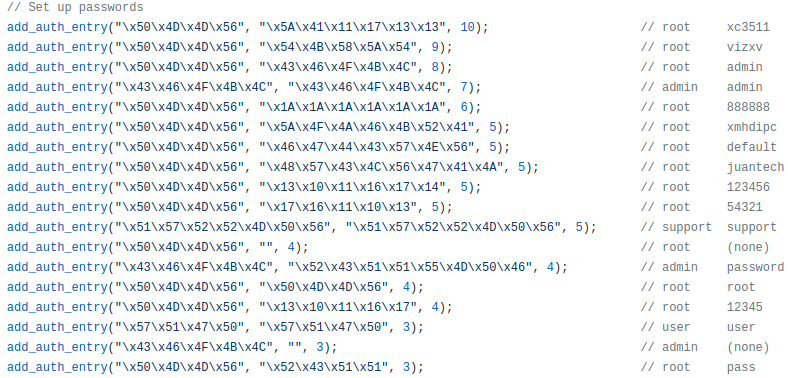
\includegraphics[width=1.2\textwidth]{mirai-dict}
 \label{fig:mirai-dict}
\end{figure}
As you can see in the figure \ref{fig:mirai-dict} the dictionnary use very simple combination of username/password to bruteforce the telnet connection.

\subsection{Other vulnerabilities}
Here his an analysis of the others major botnets and the vulnerabilities they're using.

\begin{itemize}
 \item Tsunami/Kaiten.c\autocite{tsunami} : FTP and HTTP
 \item Linux.Darlloz\autocite{darlloz} : PHP
 \item Spike/Dofloo\autocite{spike} : MIPS and ARM architectures 
\end{itemize}

This overview of the IoT botnet vulnerability usage show multiple things:
\begin{enumerate}
 \item Telnet bruteforce is the most common vulnerability used by the majority of the botnets.
 \item In order to make a botnet you need to find some vulnerabily that is common of the majority of the IoT devices
 \item A huge majority of the IoT devices are based on a Linux variant
\end{enumerate}

\chapter{Project}
\section{Analysis and choices}
The most important security breach in the IoT devices is the mean of communication and the most used in the IoT botnets is : telnet. The Goal of this project is to be able to detect a vulnerable device. 

\section{implementation}
This project in order to be able to detect the most number of vulnerable device possible is devided in three different parts. A website, an Android application and a computer ruby application.
\subsection{Web}
The choice of a web application as ben made because a web application can be accessed by anybody and permit to make the test available to anyone.

\subsection{Mobile}
A mobile aplication became something really important now. The choice of this technology permit to use a mobile device and scan for a vulnerable device easily.

\subsubsection{Android}
Android is not the only one, but it's the one that is well represented and were you can program on any operating system. Because of that Android as been the choosen to be the mobile platform of this project.

\subsubsection{Language, Development and version control}
Because of Android the language used on this mobile application is Java. Even if Android provide a support for C++ language using C++ for this application can be a bit overkill and more difficult because of there is less library for C++ on Android than with Java.\newline
The application that you can find on the Corpus (as Vulscan) as been developed on Android studio which is the IDE provided by Google.

\subsection{Computer}

\chapter{Testing}

\chapter{Conclusion and future work}
This is the conclusion of this paper, we will need to do it at the end

\printbibliography

\listoffigures

\end{document}
